\chapter{Implementation}

\section{Design}
The main objective of our project is to reduce the total number of writes. 

We have two approaches to achieve this. 
\begin{enumerate}

\item The first approach is by not replicating data to one of the replica, every time there is a write request from the client. The write is delayed for a fixed time and then initiated, this technique is called the \textbf{Lazy update.} 

\item The second is not replicating the data to any of the replicas instead log all the writes and then update the replicas after certain time. This avoids considerable program-erase cycles if same blocks are rewritten. We will call this \textbf{Logging.}

\end{enumerate}

With the first approach the replication is delayed to one of the replica nodes whereas with the second approach the delay is to all the replicas. Thus these approaches are more suitable for weak consistency applications. We wanted to design this approach on CEPH system. But due to time constraints and huge code base of CEPH we have gone ahead to design the model on a simple key, value based distributed system.

\begin{figure}[h]
    \centering
    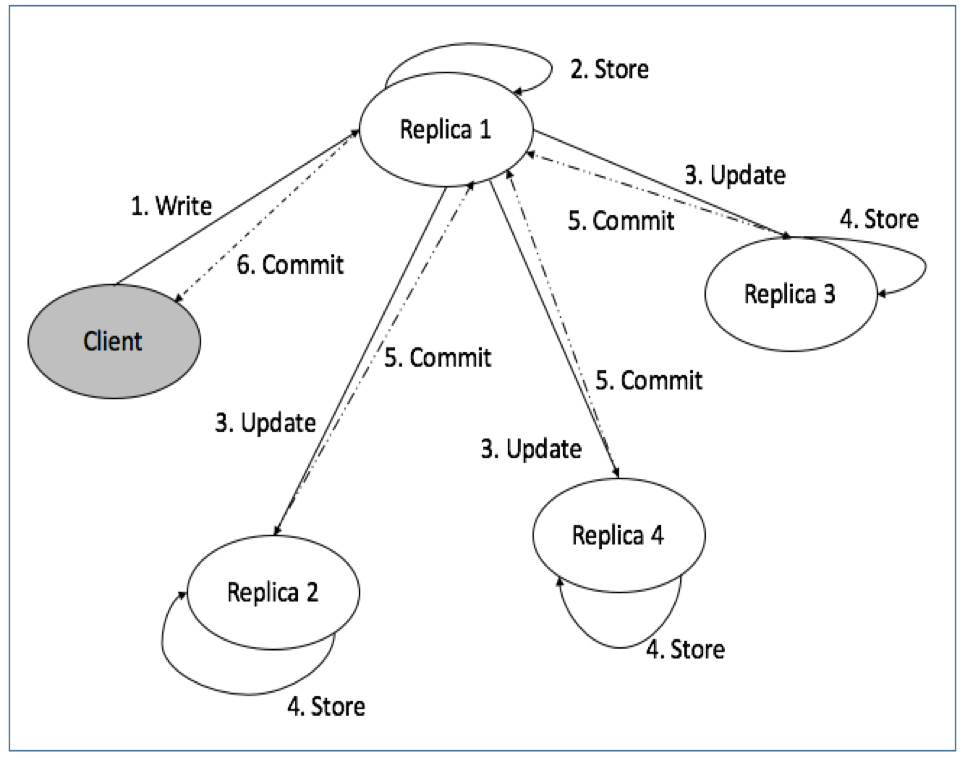
\includegraphics[width=\textwidth]{Figure1}
    \caption{Simple key, value pair Distributed System without our solution}
    \label{fig:21}
\end{figure}

Without our solution, the system would update the latest data immediately to all the replicas without any delay as shown in the figure \ref{fig:21}. Whenever there is a write request from the client, the data is replicated to all the replicas 1-4 immediately and simultaneously. This leads to more program-erase cycle thus lowering the endurance of the flash system.

\begin{figure}[h]
    \centering
    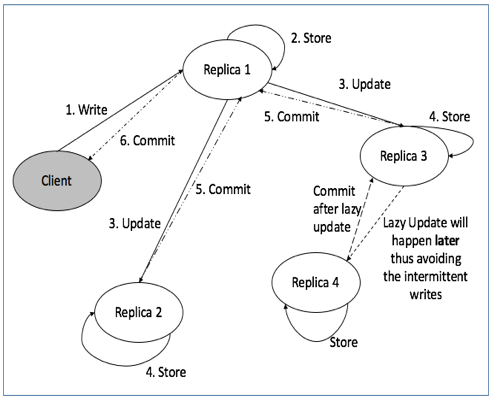
\includegraphics[width=\textwidth]{Figure2}
    \caption{Key, Value pair distributed system with lazy update on Replica 4}
    \label{fig:22}
\end{figure}

The data flow diagram with the first approach of our solution is as shown in the figure  \ref{fig:22}. 
A single replica is chosen from all the replicas for the lazy update. We have chosen Replica 4 for illustration purpose. On the event of a write request from the client, the data is replicated to all replicas immediately except for replica 4. Once all the other replicas store the new data and committed, the commit signal is sent back to the client. However, the update to replica 4 is delayed up to 2 minutes or until acceptable consistency delay. This way the number of writes to replica 4 is reduced. This increases the endurance of replica 4. With this approach, we will be able to improve the endurance of one node. The lazy update can be done to any one of the replicas for each write request on a round robin basis, thus improving endurance of all the nodes.


With the second approach, whenever a client sends a write request, it is logged in and commit signal is sent to the client. A finite number of writes is accumulated until it is actually written to all the replicas as shown in figure \ref{fig:23} below. After certain time, the accumulated writes are sent, all at once to all the replicas. This reduces the program-erase cycle of the flash system. With this approach, the intention is to improve the endurance of all the replicas.

\begin{figure}[h]
    \centering
    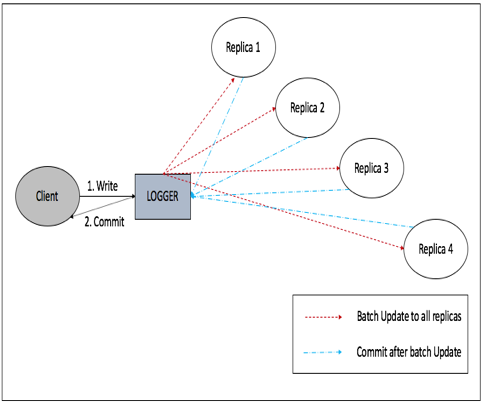
\includegraphics[width=\textwidth]{Figure3}
    \caption{Key, Value distributed system with logging for write events}
    \label{fig:23}
\end{figure}

\newpage

\section{File Structure}

The code is designed as Client Server model, where the server does the replication task and the client does the load generation. We have designed to support four instances of server code (replicas) running on different physical or virtual machine or at different network ports which is the \textbf{replicator.py} code. For the load generation we have clients running connected to different servers which is the \textbf{client.py} code. 

Apart from the above main code, the grapher.py code is used to plot the number of writes received from all the servers to get the dynamic write counts and to get the number of actual writes written from client which uses the writesfromclient.csv file.

For testing and debugging we have created the tox-quickstart and test cases files under the pytest folder. Pytest framework is used for testing. 

Refer figure \ref{fig:24} for file structure details. 

\begin{figure}[h]
    \centering
    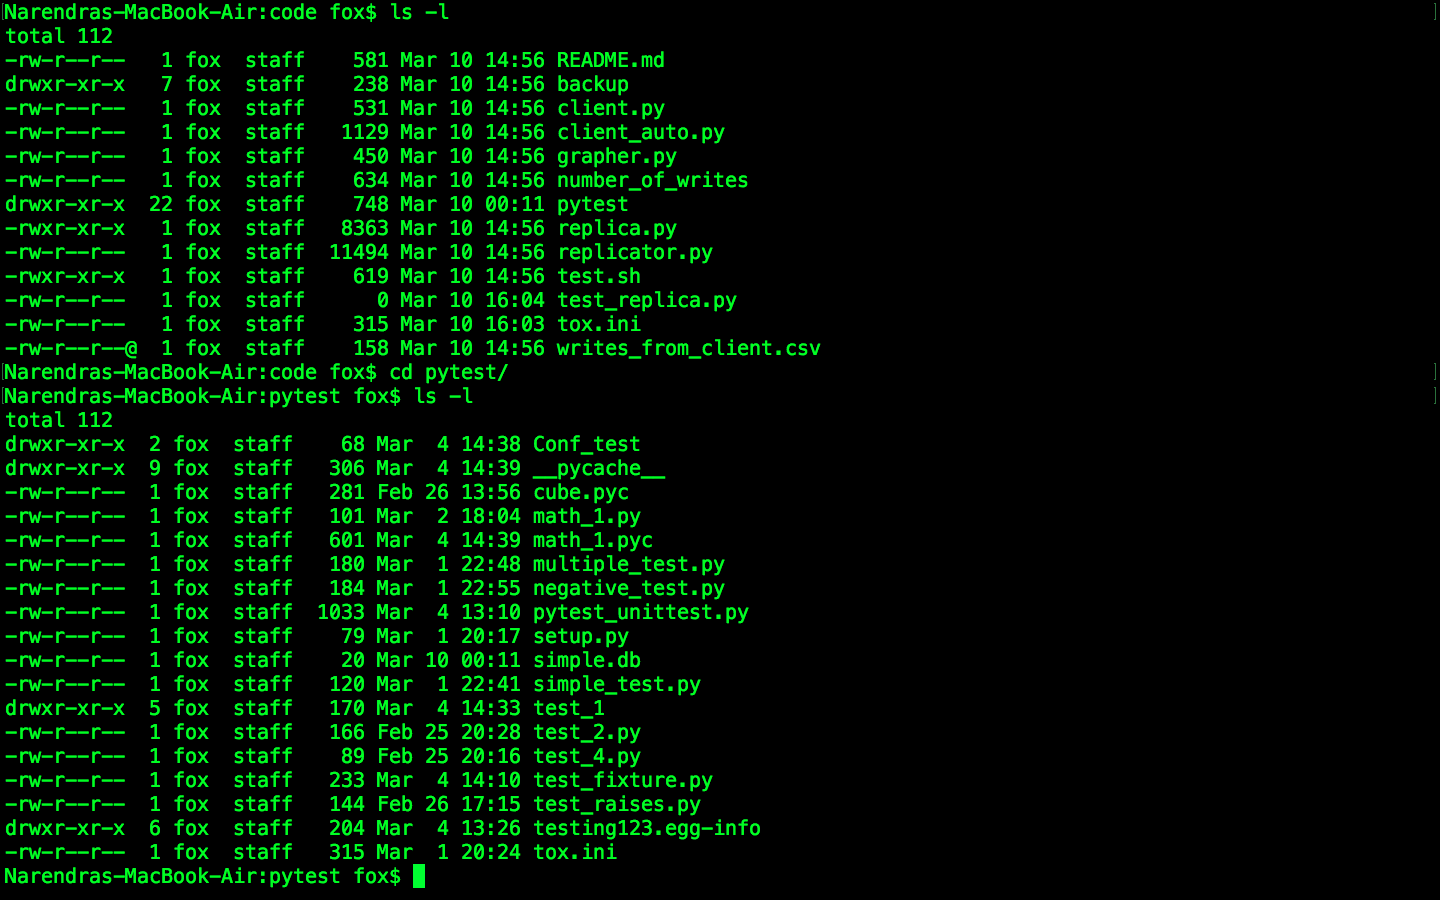
\includegraphics[width=\textwidth]{file_structure}
    \caption{File Structure}
    \label{fig:24}
\end{figure}

\section{Data Structures}

This Distributed system project is a type of dictionary data structure, where each key is unique and it stores a value. This data structure is replicated across all the disaster recovery sites using the network programming socket package which uses the TCP protocol. 

And again the same data structure which is the dictionary, is used to store the values at each of the sites. 

For this project we are using the pickledb package at each of the replicator and below are the commands supported by pickledb.

\textbf{\textit{DB operations available}}
\begin{enumerate}

\item  LOAD path dump  [Load a database from a file]

\item  SET key value [Set the string value of a key]

\item  GET key  [Get the value of a key] 

\item  GETALL [Return a list of all keys in database] 

\item  REM key [Delete a key] 

\item  APPEND key more [Add more to a key's value]

\item  LCREATE name [Create a list]

\item  LADD name value  [Add a value to a list]

\item  LGETALL name [Return all values in a list]

\item  LEXTEND name seq [Extend a list with a sequence]

\item  LGET name pos [Return one value in a list]

\item  LREM name [Remove a list and all of its values]

\item  LPOP name pos [Remove one value in a list]

\item  LLEN name [Return the length of a list]

\item  LAPPEND name pos more [Add more to a value in a list]

\item  DCREATE name [Create a dict]

\item  DADD name pair [Add a key-value pair to a dict, "pair" is a tuple]

\item  DGETALL name [Return all key-value pairs from a dict]

\item  DGET name key [Return the value for a key in a dict]

\item  DKEYS name [Return all the keys for a dict]

\item  DVALS name [Return all the values for a dict]

\item  DEXISTS name key [Determine if a key exists]

\item  DREM name [Remove a dict and all of its pairs]

\item  DPOP name key [Remove one key-value in a dict]

\item  DELDB [Delete everything from the database]

\item  DUMP [Save the database from memory to a file specified in LOAD]

\end{enumerate}

\section{Code Explanation}
It all starts by calling the python script replicator.py which will become the master replicator and the script will scan the ports and the mode of operation (Lazy update/Logging) provided by the user. 

The master replictor starts listening for the client`s connection request at the intiated port and parallely listens for all other slave replicators by using the hardcoded port numbers provided in the code. 

Later the user has to start other slave replicators on the TCP port which the master port is listening to. Thus establishing the connection between the master replicator and all the slave replicators. 

Next the client script should be started to make a connection to the master replicator. the client script is the load generator that will create the key value pairs. This generated load will be sent over the TCP socket created by the master replicator.

Once the master replicator receives the data from the client, it will be first copied to its local pickledb.  After few seconds the data will be written to the other slave replicas for disaster recovery or back up purpose. This mechanism is logging. 

Later to enhance the design, we added a mode called the lazy update which has the option for slave replicators to handle their own clients. If there is any update on the slave replicas as discussed above, data will be first written to the local pickledb and then it will be propogated to other slave nodes and the master node. But having the master node up all the time is a must, as it initiates the listening session for all the slave nodes. 

The initial design and implementation was done on a python disctionary later it was enhanced to support pickledb. Adding support for other data bases should be simple.

The difficulty was to debug the issues when we ran the code as we have distributed codes running in multiple sites.   inconsistent behaviour was seen while corelating any syncing up the multiple replication sites and clients to act as one system.  Triaging was very difficult while manual testing. To overcome this we automated the test cases and used  pytest for testing each function and debugging to see if we could achieve consistent behaviour. More about pytests and tox will be discussed later in Testing and Debugging section.

\newpage